%
%
\section{Introduction}



Pretrained foundation models (FMs) have demonstrated promising performance across a wide variety of domains in artificial intelligence including natural language processing (NLP)~\citep{devlin2018bert, radford2018improving, radford2019language, brown2020language}, computer vision (CV)~\citep{yuan2021florence, sammani2022nlx, ma2023crepe, chen2024internvl}, and sequential decision-making~\citep{chen2021decision, janner2021offline, xu2022prompting, yang2023foundation, light2024strategist, light2024pianist}. This success is attributed to FMs' impressive capability of in-context learning~\citep{dong2022survey, li2023transformers, wei2023larger, wies2024learnability} which refers to the ability to infer and understand the new (unseen) tasks provided with the context information (or prompt) and without model parameters updates.
%
Recently, in-context reinforcement learning (ICRL)~\citep{laskin2022context, grigsby2023amago, lin2023transformers, sinii2023context, zisman2023emergence, lee2024supervised, lu2024structured, wang2024transformers, dong2024context} has emerged when FMs are pretrained on sequential decision-making problems.
% {These works have promoted and witnessed the success of ICRL in generalizing to new environments/tasks without any parameter updates.}
Whereas FMs use texts as the context/prompt in NLP, ICRL treats the state-action-reward tuples as the contextual information for decision-making. 

% \red{Recent works such as Algorithm Distillation (AD), Decision Pretrained Transformer (DPT) and Decision Importance Transformer (DIT) have promoted and witnessed the success of ICRL in generalizing to new environments/tasks without any parameter updates.} \blue{Providing the names here doesn't add much. You will name them in what follows. I would just add a sentence in the previous paragraph.} 
%
However, the current state-of-the-art (SOTA) ICRL algorithms impose strict requirements on the pretraining datasets. More specifically, Algorithm Distillation (AD)~\citep{laskin2022context} requires the context to contain the complete learning history (from the initial policy to the final-trained policy) of the source (or behavior) RL algorithm for all pretraining environments. In addition, AD requires environments to have short episodes, allowing the context to capture cross-episodic information. This enables AD to learn the improvement operator of the source RL algorithm.
%
Conversely, Decision Pretrained Transformer (DPT)~\citep{lee2024supervised} {partially relaxes the} requirement on the context, permitting it to be gathered by random policies and without needing to adhere to the transition dynamics. Nevertheless, DPT necessitates the optimal policy to label an optimal action for any randomly sampled query state across all pretraining environments.
%
To explore the feasibility of ICRL in the absence of optimal policies, Decision Importance Transformer (DIT)~\citep{dong2024context} proposes to leverage the observed state-action pairs in the context data as query states and corresponding action labels. Each state-action pair within the context is assigned a weight in the training process. This weight is proportional to the return-to-go of the pair. Thus, DIT prioritizes the training on high-return pairs.
%
Despite not demanding optimal policies, DIT still requires a substantial context dataset to comprehensively cover all state-action pairs from the state and action spaces. Furthermore, DIT still mandates that more than $30\%$ of the context data comes from well-trained policies to ensure the coverage of good action labels, and the context should originate from a complete episode.
%

Notably, acquiring either optimal policies or well-trained policies across a multitude of pretraining environments in real-world scenarios can be prohibitively expensive or even intractable.
%
On the other hand, the transition data available in real-world problems—collected as the context—may not originate from a complete episode. 
%
These stringent requirements on the pretraining dataset of the SOTA ICRL algorithms severely limit their practical applications to the real world,  especially for those where the transition data exhibits high variance to train an effective policy. This work thus aims to relax these requirements by considering an untrained random policy. Although the random policy cannot solve all decision-making problems, it is worth noting that the random policy and the optimal policy select the same optimal actions in certain problems, e.g., the grid world navigation problem~\citep{laskin2022context, lee2024supervised, dong2024context} where the reward is received only upon reaching the unique goal. In these problems, the optimal action induced by both policies corresponds to navigating to the goal as quickly as possible.
%
Consequently, this paper centers on the ICRL that operates without the need for optimal (or any degree of well-trained) policies or episodic context, placing its emphasis on the scenarios under (e.g., uniform) random policies and random contexts only.
%
Our applicable domains in this work focus on the multi-armed bandits and the grid world navigation problems with a single sparse reward received only upon achieving the unique goal.

% \purple{Weiqin: Do you think the red text has the issue? If we remove this, it looks disconnected. And we didn't justify before that we can use the random policy right?} 
% \red{My suggestion is, add finish the sentence in black after the word ``policy''. Remove the ``and'' then write the following sentence:``This work aims to relax these requirements by considering untrained random policies.''
% }



\begin{figure}[ht]
\centering 
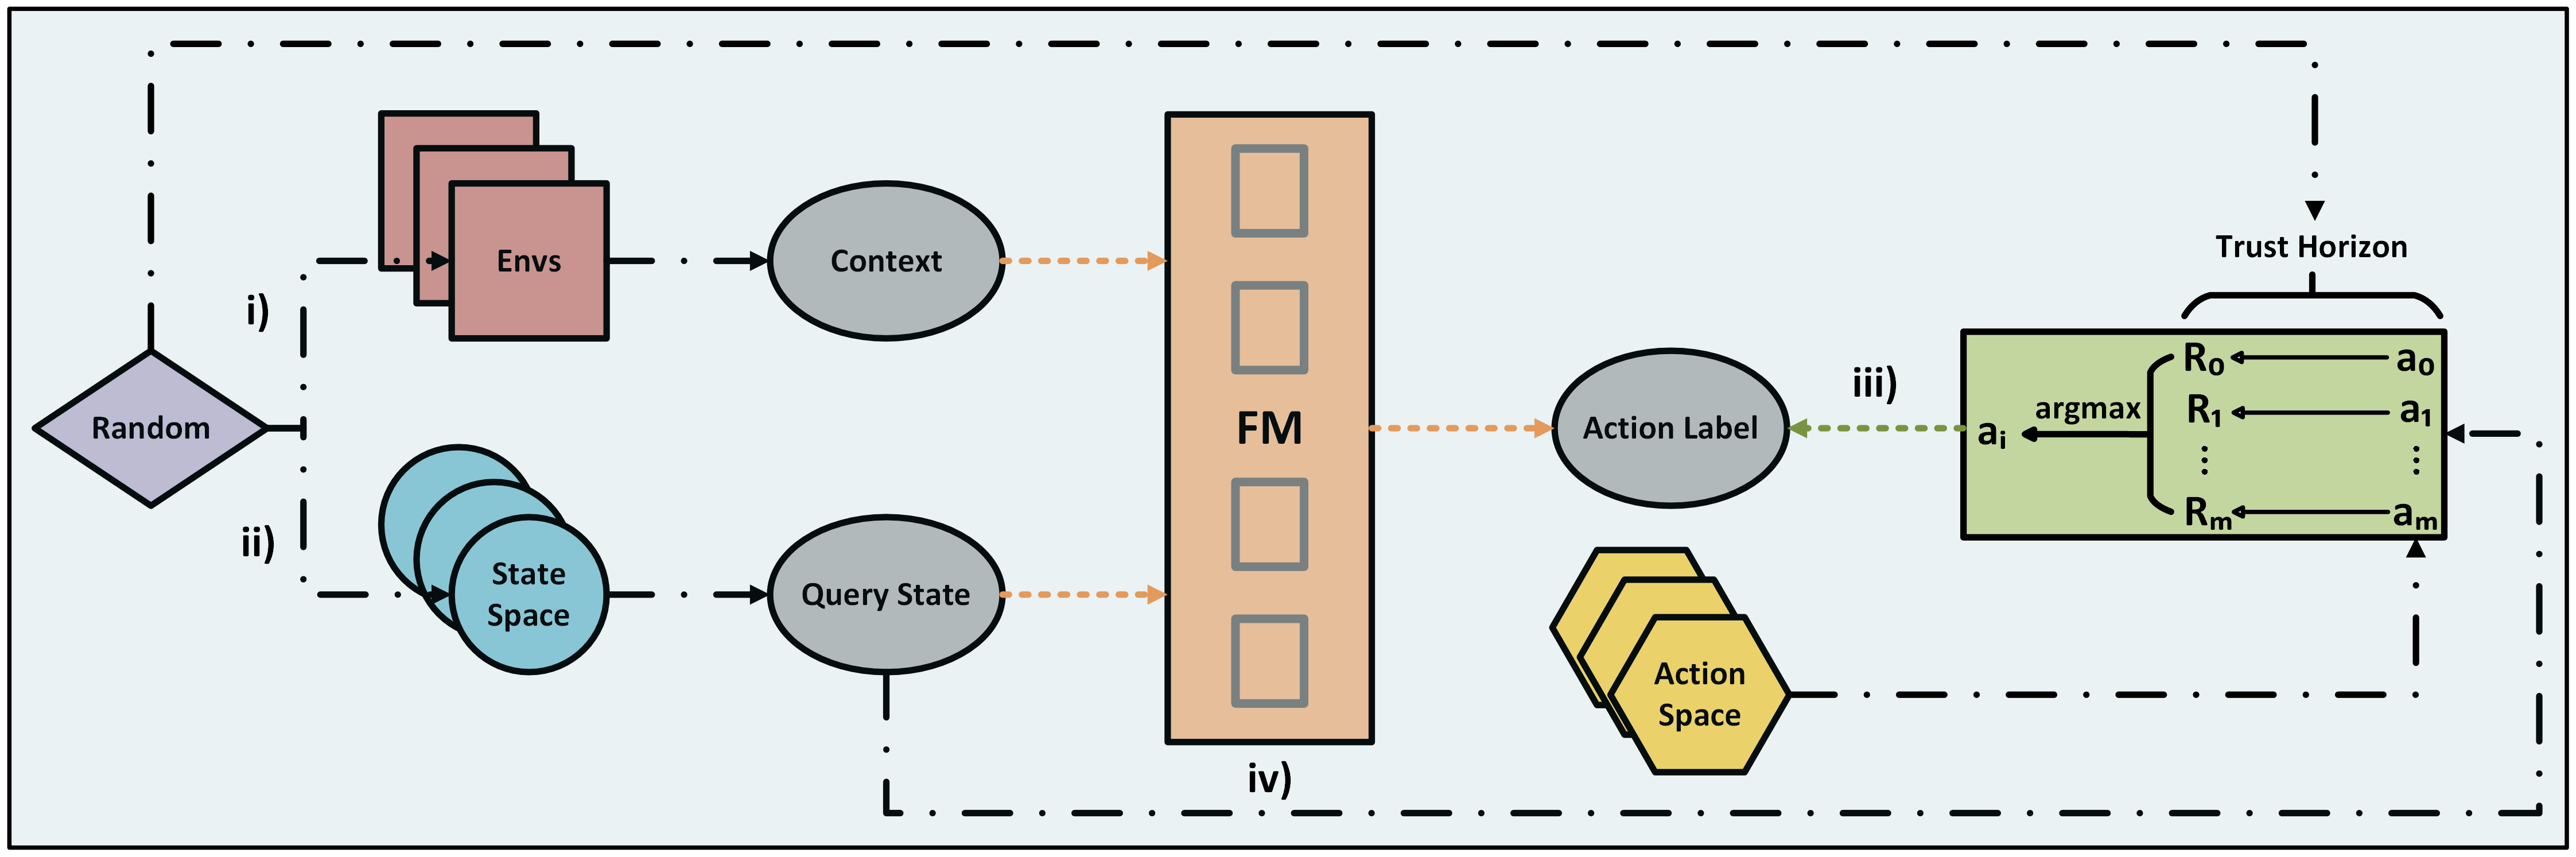
\includegraphics[width=1\linewidth]{figures/sad_schematic_new.png}  
% \Description{Schematic of State-Action Distillation.}
\caption{Schematic of the State-Action Distillation approach: i) Collecting the context by using the random policy to interact with pretraining environments. ii) Sampling a query state randomly from the state space.
%
iii) Starting from the query state and any action in action space, running trust horizons under the random policy, and distilling the action label by the action that yields the maximal return.
%
iv) Pretraining foundation models in a supervised mechanism, which predicts the action label given the context and query state.
}
\label{fig_schematic}
\end{figure}






%%%%%%%%%%%%%%%%%%%%%%%%%%%%%%%%%%%%%%%%%%%%%%%%%%%%%%%%%%%%%%%%%%%%%%%%

\subsection{Main Contributions}


The main contributions of this work are summarized as follows.
\begin{itemize}
    \item We propose a novel approach termed State-Action Distillation (SAD) to generate the pretraining dataset of ICRL under random policies. Notably, SAD distills the outstanding state-action pairs over the entire state and action spaces for the query states and corresponding action labels (refer to Figure~\ref{fig_schematic}), by executing all possible actions under the random policies within a trust horizon.
    
    \item To the best of our knowledge, SAD stands as the first method that enables effective ICRL under (e.g., uniform) random policies and random contexts.

    \item We establish the quantitative analysis of the trustworthiness as well as the performance guarantees of our SAD approach. We substantiate the efficacy of SAD by empirical results on several popular ICRL benchmark environments.
    %
    On average, SAD significantly outperforms all existing SOTA ICRL algorithms. More concretely, SAD surpasses the best baseline by $236.3\%$ in the offline evaluation and by $135.2\%$ in the online evaluation.
\end{itemize}




%%%%%%%%%%%%%%%%%%%%%%%%%%%%%%%%%%%%%%%%%%%%%%%%%%%%%%%%%%%%%%%%%%%%%%%%
